% Copyright (c) 2013 by the University of Waikato, Hamilton, NZ. 
% This work is made available under the terms of the 
% Creative Commons Attribution-ShareAlike 3.0 license, 
% http://creativecommons.org/licenses/by-sa/3.0/. 
%
% Version: $Revision$

\documentclass[a4paper]{book}

\usepackage{wrapfig}
\usepackage{graphicx}
\usepackage{hyperref}
\usepackage{multirow}
\usepackage{scalefnt}
\usepackage{tikz}

% watermark -- for draft stage
\usepackage[firstpage]{draftwatermark}
\SetWatermarkLightness{0.9}
\SetWatermarkScale{5}

% Copyright (c) 2009 by the University of Waikato, Hamilton, NZ. 
% This work is made available under the terms of the 
% Creative Commons Attribution-ShareAlike 3.0 license, 
% http://creativecommons.org/licenses/by-sa/3.0/. 
%
% Version: $Revision: 2916 $

\newenvironment{tight_itemize}{
\begin{itemize}
  \setlength{\itemsep}{1pt}
  \setlength{\parskip}{0pt}
  \setlength{\parsep}{0pt}}{\end{itemize}
}

\newenvironment{tight_enumerate}{
\begin{enumerate}
  \setlength{\itemsep}{1pt}
  \setlength{\parskip}{0pt}
  \setlength{\parsep}{0pt}}{\end{enumerate}
}

% if you just need a simple heading
% Usage:
%   \heading{the text of the heading}
\newcommand{\heading}[1]{
  \vspace{0.3cm} \noindent \textbf{#1} \newline
}

\newcommand{\icon}[1]{\tikz[baseline=-3pt]\node[inner sep=0pt,outer sep=0pt]{\includegraphics[height=1.1em]{#1}};}


\title{
  \textbf{ADAMS} \\
  {\Large \textbf{A}dvanced \textbf{D}ata mining \textbf{A}nd \textbf{M}achine
  learning \textbf{S}ystem} \\
  {\Large Module: adams-geotools} \\
  \vspace{1cm}
  
\includegraphics[width=2cm]{images/geotools-module.png} \\
}
\author{
  Peter Reutemann
}

\setcounter{secnumdepth}{3}
\setcounter{tocdepth}{3}

\begin{document}

\begin{titlepage}
\maketitle

\thispagestyle{empty}
\center
\begin{table}[b]
	\begin{tabular}{c l l}
		\parbox[c][2cm]{2cm}{\copyright 2013} &
		\parbox[c][2cm]{5cm}{
\includegraphics[width=5cm]{images/coat_of_arms.pdf}} \\
	\end{tabular}
	
\includegraphics[width=12cm]{images/cc.png} \\
\end{table}

\end{titlepage}

\tableofcontents
\listoffigures
%\listoftables

%%%%%%%%%%%%%%%%%%%%%%%%%%%%%%%%%%%
\chapter{Introduction}
\textit{GeoTools} is an LGPL-licensed\footnote{\url{http://www.gnu.org/licenses/lgpl-2.1.html}{}} 
set of libraries for geospatial data.

%%%%%%%%%%%%%%%%%%%%%%%%%%%%%%%%%%%
\chapter{Flow}
The following actors are available:
\begin{tight_itemize}
	\item \textit{GeoToolsLayerFileReader} -- transformer for reading shape 
	and raster files (e.g., TIFF) and turns them into layers.
	\item \textit{GeoToolsLayerFileWriter} -- sink for writing layers to disk.
	\item \textit{GeoToolsMapDisplay} -- sink for displaying maps, i.e., layers.
\end{tight_itemize}
The following conversions are available:
\begin{tight_itemize}
	\item \textit{SpreadSheetToGeoToolsLayer} -- turns a spreadsheet into a 
	layer that can be displayed with a \textit{GeoToolsMapDisplay} sink.
\end{tight_itemize}

%%%%%%%%%%%%%%%%%%%%%%%%%%%%%%%%%%%
\chapter{Data}
Publicly available datasets to be used with GeoTools can be obtained, for
instance, from \textit{Natural Earth} \cite{naturalearth}.

%%%%%%%%%%%%%%%%%%%%%%%%%%%%%%%%%%%
\chapter{Tools}
The \textit{Map display} tool can be found in the \textit{Visualization} menu
of the ADAMS main menu. It allows you to load files of format shapefile and 
geotiff\footnote{Changes to the way the JRE loads images seem to result now
in errors as mentioned \url{https://www.liferay.com/community/forums/-/message_boards/message/26368932}{here}.}.
You can load as many layers as you want to, enable/disable and remove them.
Figure \ref{mapdisplay-vector} shows the tool with just a single vector layer.

\begin{figure}[htb]
  \centering
  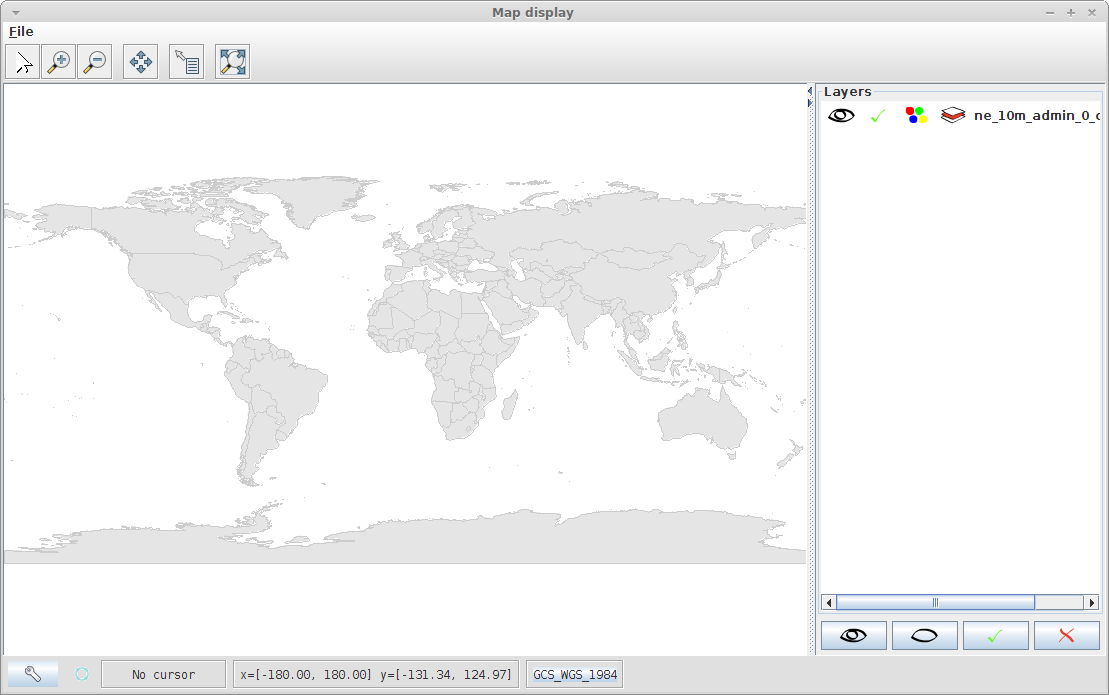
\includegraphics[width=10.0cm]{images/map_vector.png}
  \caption{Map display showing a vector shapefile}
  \label{mapdisplay-vector}
\end{figure}

%%%%%%%%%%%%%%%%%%%%%%%%%%%%%%%%%%%
% Copyright (c) 2009-2012 by the University of Waikato, Hamilton, NZ. 
% This work is made available under the terms of the 
% Creative Commons Attribution-ShareAlike 4.0 license,
% http://creativecommons.org/licenses/by-sa/4.0/.
%
% Version: $Revision$

\begin{thebibliography}{999}
	% to make the bibliography appear in the TOC
	\addcontentsline{toc}{chapter}{Bibliography}

    % references
	\bibitem{adams}
		\textit{ADAMS} -- Advanced Data mining and Machine learning System \\
		\url{https://adams.cms.waikato.ac.nz/}{}
		
	\bibitem{dl4j}
		\textit{deeplearning4j} -- open-source, distributed,
		deep-learning library for the JVM. \\
		\url{http://deeplearning4j.org/}{}

	\bibitem{json}
		\textit{JSON} -- JavaScript Object Notation is a lightweight data-interchange format \\
		\url{http://json.org/}{}

	\bibitem{yaml}
		\textit{YAML} -- is a human friendly data serialization
                standard for all programming languages. \\
		\url{http://yaml.org/}{}

\end{thebibliography}


\end{document}
